
% Default to the notebook output style

    


% Inherit from the specified cell style.




    
\documentclass[11pt]{article}

    
    
    \usepackage[T1]{fontenc}
    % Nicer default font (+ math font) than Computer Modern for most use cases
    \usepackage{mathpazo}

    % Basic figure setup, for now with no caption control since it's done
    % automatically by Pandoc (which extracts ![](path) syntax from Markdown).
    \usepackage{graphicx}
    % We will generate all images so they have a width \maxwidth. This means
    % that they will get their normal width if they fit onto the page, but
    % are scaled down if they would overflow the margins.
    \makeatletter
    \def\maxwidth{\ifdim\Gin@nat@width>\linewidth\linewidth
    \else\Gin@nat@width\fi}
    \makeatother
    \let\Oldincludegraphics\includegraphics
    % Set max figure width to be 80% of text width, for now hardcoded.
    \renewcommand{\includegraphics}[1]{\Oldincludegraphics[width=.8\maxwidth]{#1}}
    % Ensure that by default, figures have no caption (until we provide a
    % proper Figure object with a Caption API and a way to capture that
    % in the conversion process - todo).
    \usepackage{caption}
    \DeclareCaptionLabelFormat{nolabel}{}
    \captionsetup{labelformat=nolabel}

    \usepackage{adjustbox} % Used to constrain images to a maximum size 
    \usepackage{xcolor} % Allow colors to be defined
    \usepackage{enumerate} % Needed for markdown enumerations to work
    \usepackage{geometry} % Used to adjust the document margins
    \usepackage{amsmath} % Equations
    \usepackage{amssymb} % Equations
    \usepackage{textcomp} % defines textquotesingle
    % Hack from http://tex.stackexchange.com/a/47451/13684:
    \AtBeginDocument{%
        \def\PYZsq{\textquotesingle}% Upright quotes in Pygmentized code
    }
    \usepackage{upquote} % Upright quotes for verbatim code
    \usepackage{eurosym} % defines \euro
    \usepackage[mathletters]{ucs} % Extended unicode (utf-8) support
    \usepackage[utf8x]{inputenc} % Allow utf-8 characters in the tex document
    \usepackage{fancyvrb} % verbatim replacement that allows latex
    \usepackage{grffile} % extends the file name processing of package graphics 
                         % to support a larger range 
    % The hyperref package gives us a pdf with properly built
    % internal navigation ('pdf bookmarks' for the table of contents,
    % internal cross-reference links, web links for URLs, etc.)
    \usepackage{hyperref}
    \usepackage{longtable} % longtable support required by pandoc >1.10
    \usepackage{booktabs}  % table support for pandoc > 1.12.2
    \usepackage[inline]{enumitem} % IRkernel/repr support (it uses the enumerate* environment)
    \usepackage[normalem]{ulem} % ulem is needed to support strikethroughs (\sout)
                                % normalem makes italics be italics, not underlines
    

    
    
    % Colors for the hyperref package
    \definecolor{urlcolor}{rgb}{0,.145,.698}
    \definecolor{linkcolor}{rgb}{.71,0.21,0.01}
    \definecolor{citecolor}{rgb}{.12,.54,.11}

    % ANSI colors
    \definecolor{ansi-black}{HTML}{3E424D}
    \definecolor{ansi-black-intense}{HTML}{282C36}
    \definecolor{ansi-red}{HTML}{E75C58}
    \definecolor{ansi-red-intense}{HTML}{B22B31}
    \definecolor{ansi-green}{HTML}{00A250}
    \definecolor{ansi-green-intense}{HTML}{007427}
    \definecolor{ansi-yellow}{HTML}{DDB62B}
    \definecolor{ansi-yellow-intense}{HTML}{B27D12}
    \definecolor{ansi-blue}{HTML}{208FFB}
    \definecolor{ansi-blue-intense}{HTML}{0065CA}
    \definecolor{ansi-magenta}{HTML}{D160C4}
    \definecolor{ansi-magenta-intense}{HTML}{A03196}
    \definecolor{ansi-cyan}{HTML}{60C6C8}
    \definecolor{ansi-cyan-intense}{HTML}{258F8F}
    \definecolor{ansi-white}{HTML}{C5C1B4}
    \definecolor{ansi-white-intense}{HTML}{A1A6B2}

    % commands and environments needed by pandoc snippets
    % extracted from the output of `pandoc -s`
    \providecommand{\tightlist}{%
      \setlength{\itemsep}{0pt}\setlength{\parskip}{0pt}}
    \DefineVerbatimEnvironment{Highlighting}{Verbatim}{commandchars=\\\{\}}
    % Add ',fontsize=\small' for more characters per line
    \newenvironment{Shaded}{}{}
    \newcommand{\KeywordTok}[1]{\textcolor[rgb]{0.00,0.44,0.13}{\textbf{{#1}}}}
    \newcommand{\DataTypeTok}[1]{\textcolor[rgb]{0.56,0.13,0.00}{{#1}}}
    \newcommand{\DecValTok}[1]{\textcolor[rgb]{0.25,0.63,0.44}{{#1}}}
    \newcommand{\BaseNTok}[1]{\textcolor[rgb]{0.25,0.63,0.44}{{#1}}}
    \newcommand{\FloatTok}[1]{\textcolor[rgb]{0.25,0.63,0.44}{{#1}}}
    \newcommand{\CharTok}[1]{\textcolor[rgb]{0.25,0.44,0.63}{{#1}}}
    \newcommand{\StringTok}[1]{\textcolor[rgb]{0.25,0.44,0.63}{{#1}}}
    \newcommand{\CommentTok}[1]{\textcolor[rgb]{0.38,0.63,0.69}{\textit{{#1}}}}
    \newcommand{\OtherTok}[1]{\textcolor[rgb]{0.00,0.44,0.13}{{#1}}}
    \newcommand{\AlertTok}[1]{\textcolor[rgb]{1.00,0.00,0.00}{\textbf{{#1}}}}
    \newcommand{\FunctionTok}[1]{\textcolor[rgb]{0.02,0.16,0.49}{{#1}}}
    \newcommand{\RegionMarkerTok}[1]{{#1}}
    \newcommand{\ErrorTok}[1]{\textcolor[rgb]{1.00,0.00,0.00}{\textbf{{#1}}}}
    \newcommand{\NormalTok}[1]{{#1}}
    
    % Additional commands for more recent versions of Pandoc
    \newcommand{\ConstantTok}[1]{\textcolor[rgb]{0.53,0.00,0.00}{{#1}}}
    \newcommand{\SpecialCharTok}[1]{\textcolor[rgb]{0.25,0.44,0.63}{{#1}}}
    \newcommand{\VerbatimStringTok}[1]{\textcolor[rgb]{0.25,0.44,0.63}{{#1}}}
    \newcommand{\SpecialStringTok}[1]{\textcolor[rgb]{0.73,0.40,0.53}{{#1}}}
    \newcommand{\ImportTok}[1]{{#1}}
    \newcommand{\DocumentationTok}[1]{\textcolor[rgb]{0.73,0.13,0.13}{\textit{{#1}}}}
    \newcommand{\AnnotationTok}[1]{\textcolor[rgb]{0.38,0.63,0.69}{\textbf{\textit{{#1}}}}}
    \newcommand{\CommentVarTok}[1]{\textcolor[rgb]{0.38,0.63,0.69}{\textbf{\textit{{#1}}}}}
    \newcommand{\VariableTok}[1]{\textcolor[rgb]{0.10,0.09,0.49}{{#1}}}
    \newcommand{\ControlFlowTok}[1]{\textcolor[rgb]{0.00,0.44,0.13}{\textbf{{#1}}}}
    \newcommand{\OperatorTok}[1]{\textcolor[rgb]{0.40,0.40,0.40}{{#1}}}
    \newcommand{\BuiltInTok}[1]{{#1}}
    \newcommand{\ExtensionTok}[1]{{#1}}
    \newcommand{\PreprocessorTok}[1]{\textcolor[rgb]{0.74,0.48,0.00}{{#1}}}
    \newcommand{\AttributeTok}[1]{\textcolor[rgb]{0.49,0.56,0.16}{{#1}}}
    \newcommand{\InformationTok}[1]{\textcolor[rgb]{0.38,0.63,0.69}{\textbf{\textit{{#1}}}}}
    \newcommand{\WarningTok}[1]{\textcolor[rgb]{0.38,0.63,0.69}{\textbf{\textit{{#1}}}}}
    
    
    % Define a nice break command that doesn't care if a line doesn't already
    % exist.
    \def\br{\hspace*{\fill} \\* }
    % Math Jax compatability definitions
    \def\gt{>}
    \def\lt{<}
    % Document parameters
    \title{Report}
    
    
    

    % Pygments definitions
    
\makeatletter
\def\PY@reset{\let\PY@it=\relax \let\PY@bf=\relax%
    \let\PY@ul=\relax \let\PY@tc=\relax%
    \let\PY@bc=\relax \let\PY@ff=\relax}
\def\PY@tok#1{\csname PY@tok@#1\endcsname}
\def\PY@toks#1+{\ifx\relax#1\empty\else%
    \PY@tok{#1}\expandafter\PY@toks\fi}
\def\PY@do#1{\PY@bc{\PY@tc{\PY@ul{%
    \PY@it{\PY@bf{\PY@ff{#1}}}}}}}
\def\PY#1#2{\PY@reset\PY@toks#1+\relax+\PY@do{#2}}

\expandafter\def\csname PY@tok@vi\endcsname{\def\PY@tc##1{\textcolor[rgb]{0.10,0.09,0.49}{##1}}}
\expandafter\def\csname PY@tok@m\endcsname{\def\PY@tc##1{\textcolor[rgb]{0.40,0.40,0.40}{##1}}}
\expandafter\def\csname PY@tok@gp\endcsname{\let\PY@bf=\textbf\def\PY@tc##1{\textcolor[rgb]{0.00,0.00,0.50}{##1}}}
\expandafter\def\csname PY@tok@nn\endcsname{\let\PY@bf=\textbf\def\PY@tc##1{\textcolor[rgb]{0.00,0.00,1.00}{##1}}}
\expandafter\def\csname PY@tok@kn\endcsname{\let\PY@bf=\textbf\def\PY@tc##1{\textcolor[rgb]{0.00,0.50,0.00}{##1}}}
\expandafter\def\csname PY@tok@na\endcsname{\def\PY@tc##1{\textcolor[rgb]{0.49,0.56,0.16}{##1}}}
\expandafter\def\csname PY@tok@k\endcsname{\let\PY@bf=\textbf\def\PY@tc##1{\textcolor[rgb]{0.00,0.50,0.00}{##1}}}
\expandafter\def\csname PY@tok@no\endcsname{\def\PY@tc##1{\textcolor[rgb]{0.53,0.00,0.00}{##1}}}
\expandafter\def\csname PY@tok@mb\endcsname{\def\PY@tc##1{\textcolor[rgb]{0.40,0.40,0.40}{##1}}}
\expandafter\def\csname PY@tok@il\endcsname{\def\PY@tc##1{\textcolor[rgb]{0.40,0.40,0.40}{##1}}}
\expandafter\def\csname PY@tok@cpf\endcsname{\let\PY@it=\textit\def\PY@tc##1{\textcolor[rgb]{0.25,0.50,0.50}{##1}}}
\expandafter\def\csname PY@tok@vm\endcsname{\def\PY@tc##1{\textcolor[rgb]{0.10,0.09,0.49}{##1}}}
\expandafter\def\csname PY@tok@gh\endcsname{\let\PY@bf=\textbf\def\PY@tc##1{\textcolor[rgb]{0.00,0.00,0.50}{##1}}}
\expandafter\def\csname PY@tok@vc\endcsname{\def\PY@tc##1{\textcolor[rgb]{0.10,0.09,0.49}{##1}}}
\expandafter\def\csname PY@tok@vg\endcsname{\def\PY@tc##1{\textcolor[rgb]{0.10,0.09,0.49}{##1}}}
\expandafter\def\csname PY@tok@cs\endcsname{\let\PY@it=\textit\def\PY@tc##1{\textcolor[rgb]{0.25,0.50,0.50}{##1}}}
\expandafter\def\csname PY@tok@gt\endcsname{\def\PY@tc##1{\textcolor[rgb]{0.00,0.27,0.87}{##1}}}
\expandafter\def\csname PY@tok@c\endcsname{\let\PY@it=\textit\def\PY@tc##1{\textcolor[rgb]{0.25,0.50,0.50}{##1}}}
\expandafter\def\csname PY@tok@nl\endcsname{\def\PY@tc##1{\textcolor[rgb]{0.63,0.63,0.00}{##1}}}
\expandafter\def\csname PY@tok@gs\endcsname{\let\PY@bf=\textbf}
\expandafter\def\csname PY@tok@s2\endcsname{\def\PY@tc##1{\textcolor[rgb]{0.73,0.13,0.13}{##1}}}
\expandafter\def\csname PY@tok@cp\endcsname{\def\PY@tc##1{\textcolor[rgb]{0.74,0.48,0.00}{##1}}}
\expandafter\def\csname PY@tok@ow\endcsname{\let\PY@bf=\textbf\def\PY@tc##1{\textcolor[rgb]{0.67,0.13,1.00}{##1}}}
\expandafter\def\csname PY@tok@gr\endcsname{\def\PY@tc##1{\textcolor[rgb]{1.00,0.00,0.00}{##1}}}
\expandafter\def\csname PY@tok@c1\endcsname{\let\PY@it=\textit\def\PY@tc##1{\textcolor[rgb]{0.25,0.50,0.50}{##1}}}
\expandafter\def\csname PY@tok@si\endcsname{\let\PY@bf=\textbf\def\PY@tc##1{\textcolor[rgb]{0.73,0.40,0.53}{##1}}}
\expandafter\def\csname PY@tok@s\endcsname{\def\PY@tc##1{\textcolor[rgb]{0.73,0.13,0.13}{##1}}}
\expandafter\def\csname PY@tok@fm\endcsname{\def\PY@tc##1{\textcolor[rgb]{0.00,0.00,1.00}{##1}}}
\expandafter\def\csname PY@tok@ss\endcsname{\def\PY@tc##1{\textcolor[rgb]{0.10,0.09,0.49}{##1}}}
\expandafter\def\csname PY@tok@nc\endcsname{\let\PY@bf=\textbf\def\PY@tc##1{\textcolor[rgb]{0.00,0.00,1.00}{##1}}}
\expandafter\def\csname PY@tok@kt\endcsname{\def\PY@tc##1{\textcolor[rgb]{0.69,0.00,0.25}{##1}}}
\expandafter\def\csname PY@tok@mf\endcsname{\def\PY@tc##1{\textcolor[rgb]{0.40,0.40,0.40}{##1}}}
\expandafter\def\csname PY@tok@nf\endcsname{\def\PY@tc##1{\textcolor[rgb]{0.00,0.00,1.00}{##1}}}
\expandafter\def\csname PY@tok@sx\endcsname{\def\PY@tc##1{\textcolor[rgb]{0.00,0.50,0.00}{##1}}}
\expandafter\def\csname PY@tok@sh\endcsname{\def\PY@tc##1{\textcolor[rgb]{0.73,0.13,0.13}{##1}}}
\expandafter\def\csname PY@tok@sc\endcsname{\def\PY@tc##1{\textcolor[rgb]{0.73,0.13,0.13}{##1}}}
\expandafter\def\csname PY@tok@nb\endcsname{\def\PY@tc##1{\textcolor[rgb]{0.00,0.50,0.00}{##1}}}
\expandafter\def\csname PY@tok@ch\endcsname{\let\PY@it=\textit\def\PY@tc##1{\textcolor[rgb]{0.25,0.50,0.50}{##1}}}
\expandafter\def\csname PY@tok@sr\endcsname{\def\PY@tc##1{\textcolor[rgb]{0.73,0.40,0.53}{##1}}}
\expandafter\def\csname PY@tok@kr\endcsname{\let\PY@bf=\textbf\def\PY@tc##1{\textcolor[rgb]{0.00,0.50,0.00}{##1}}}
\expandafter\def\csname PY@tok@se\endcsname{\let\PY@bf=\textbf\def\PY@tc##1{\textcolor[rgb]{0.73,0.40,0.13}{##1}}}
\expandafter\def\csname PY@tok@kp\endcsname{\def\PY@tc##1{\textcolor[rgb]{0.00,0.50,0.00}{##1}}}
\expandafter\def\csname PY@tok@bp\endcsname{\def\PY@tc##1{\textcolor[rgb]{0.00,0.50,0.00}{##1}}}
\expandafter\def\csname PY@tok@nd\endcsname{\def\PY@tc##1{\textcolor[rgb]{0.67,0.13,1.00}{##1}}}
\expandafter\def\csname PY@tok@sa\endcsname{\def\PY@tc##1{\textcolor[rgb]{0.73,0.13,0.13}{##1}}}
\expandafter\def\csname PY@tok@gd\endcsname{\def\PY@tc##1{\textcolor[rgb]{0.63,0.00,0.00}{##1}}}
\expandafter\def\csname PY@tok@mh\endcsname{\def\PY@tc##1{\textcolor[rgb]{0.40,0.40,0.40}{##1}}}
\expandafter\def\csname PY@tok@sb\endcsname{\def\PY@tc##1{\textcolor[rgb]{0.73,0.13,0.13}{##1}}}
\expandafter\def\csname PY@tok@ne\endcsname{\let\PY@bf=\textbf\def\PY@tc##1{\textcolor[rgb]{0.82,0.25,0.23}{##1}}}
\expandafter\def\csname PY@tok@nv\endcsname{\def\PY@tc##1{\textcolor[rgb]{0.10,0.09,0.49}{##1}}}
\expandafter\def\csname PY@tok@go\endcsname{\def\PY@tc##1{\textcolor[rgb]{0.53,0.53,0.53}{##1}}}
\expandafter\def\csname PY@tok@nt\endcsname{\let\PY@bf=\textbf\def\PY@tc##1{\textcolor[rgb]{0.00,0.50,0.00}{##1}}}
\expandafter\def\csname PY@tok@dl\endcsname{\def\PY@tc##1{\textcolor[rgb]{0.73,0.13,0.13}{##1}}}
\expandafter\def\csname PY@tok@w\endcsname{\def\PY@tc##1{\textcolor[rgb]{0.73,0.73,0.73}{##1}}}
\expandafter\def\csname PY@tok@cm\endcsname{\let\PY@it=\textit\def\PY@tc##1{\textcolor[rgb]{0.25,0.50,0.50}{##1}}}
\expandafter\def\csname PY@tok@s1\endcsname{\def\PY@tc##1{\textcolor[rgb]{0.73,0.13,0.13}{##1}}}
\expandafter\def\csname PY@tok@err\endcsname{\def\PY@bc##1{\setlength{\fboxsep}{0pt}\fcolorbox[rgb]{1.00,0.00,0.00}{1,1,1}{\strut ##1}}}
\expandafter\def\csname PY@tok@ge\endcsname{\let\PY@it=\textit}
\expandafter\def\csname PY@tok@kc\endcsname{\let\PY@bf=\textbf\def\PY@tc##1{\textcolor[rgb]{0.00,0.50,0.00}{##1}}}
\expandafter\def\csname PY@tok@sd\endcsname{\let\PY@it=\textit\def\PY@tc##1{\textcolor[rgb]{0.73,0.13,0.13}{##1}}}
\expandafter\def\csname PY@tok@gi\endcsname{\def\PY@tc##1{\textcolor[rgb]{0.00,0.63,0.00}{##1}}}
\expandafter\def\csname PY@tok@kd\endcsname{\let\PY@bf=\textbf\def\PY@tc##1{\textcolor[rgb]{0.00,0.50,0.00}{##1}}}
\expandafter\def\csname PY@tok@mo\endcsname{\def\PY@tc##1{\textcolor[rgb]{0.40,0.40,0.40}{##1}}}
\expandafter\def\csname PY@tok@mi\endcsname{\def\PY@tc##1{\textcolor[rgb]{0.40,0.40,0.40}{##1}}}
\expandafter\def\csname PY@tok@gu\endcsname{\let\PY@bf=\textbf\def\PY@tc##1{\textcolor[rgb]{0.50,0.00,0.50}{##1}}}
\expandafter\def\csname PY@tok@ni\endcsname{\let\PY@bf=\textbf\def\PY@tc##1{\textcolor[rgb]{0.60,0.60,0.60}{##1}}}
\expandafter\def\csname PY@tok@o\endcsname{\def\PY@tc##1{\textcolor[rgb]{0.40,0.40,0.40}{##1}}}

\def\PYZbs{\char`\\}
\def\PYZus{\char`\_}
\def\PYZob{\char`\{}
\def\PYZcb{\char`\}}
\def\PYZca{\char`\^}
\def\PYZam{\char`\&}
\def\PYZlt{\char`\<}
\def\PYZgt{\char`\>}
\def\PYZsh{\char`\#}
\def\PYZpc{\char`\%}
\def\PYZdl{\char`\$}
\def\PYZhy{\char`\-}
\def\PYZsq{\char`\'}
\def\PYZdq{\char`\"}
\def\PYZti{\char`\~}
% for compatibility with earlier versions
\def\PYZat{@}
\def\PYZlb{[}
\def\PYZrb{]}
\makeatother


    % Exact colors from NB
    \definecolor{incolor}{rgb}{0.0, 0.0, 0.5}
    \definecolor{outcolor}{rgb}{0.545, 0.0, 0.0}



    
    % Prevent overflowing lines due to hard-to-break entities
    \sloppy 
    % Setup hyperref package
    \hypersetup{
      breaklinks=true,  % so long urls are correctly broken across lines
      colorlinks=true,
      urlcolor=urlcolor,
      linkcolor=linkcolor,
      citecolor=citecolor,
      }
    % Slightly bigger margins than the latex defaults
    
    \geometry{verbose,tmargin=1in,bmargin=1in,lmargin=1in,rmargin=1in}
    
    

    \begin{document}
    
    
    \maketitle
    
    

    
    \section{8 bit RISC Microprocessor}\label{bit-risc-microprocessor}

\textbf{Author: Varun Sundar, EE16B068.}

\emph{Done as a part of semester project for EE2016 (Fall 2017)}

This serves as both a documentation and a report for the project.
Architecture based on Harvard RISC Architecture.

Block Diagram

\begin{figure}
\centering
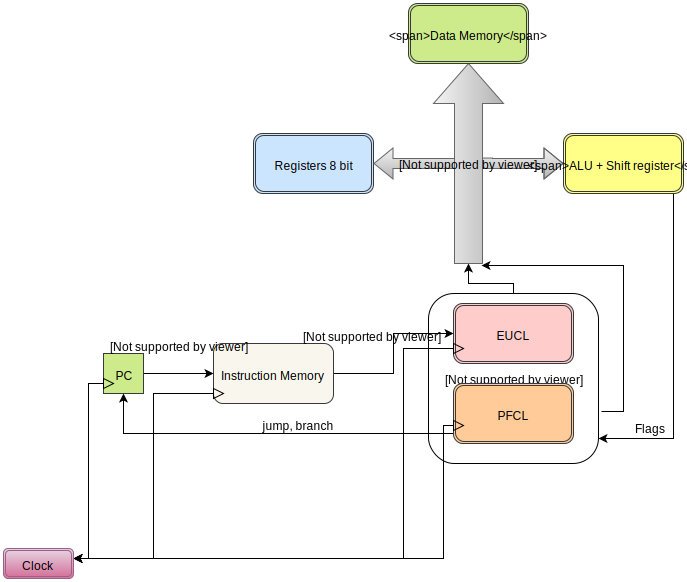
\includegraphics{./Block_diag_8_bit.svg}
\caption{\emph{Block Diagram}}
\end{figure}

\begin{center}\rule{0.5\linewidth}{\linethickness}\end{center}

\subsubsection{General Structure:}\label{general-structure}

\begin{itemize}
\tightlist
\item
  8 bit processor.
\item
  8 bit Program counter.
\item
  16 bit IMEM output.
\item
  8 registers R0 to R7, of 8 bits each. \_\_\_\_\_\_\_\_\_
\end{itemize}

\subsubsection{Module Descriptions:}\label{module-descriptions}

\begin{enumerate}
\def\labelenumi{\arabic{enumi}.}
\item ~
  \paragraph{Instruction memory}\label{instruction-memory}

  This is be a combinational unit - it takes just the address bus (8 bit
  value) as input, and gives out a 16-bit value that is the instruction
  to be decoded. The address is provided by the Program Counter (PC).
\item ~
  \paragraph{Program Counter}\label{program-counter}

  8 bit register. Under normal operations, will always increment by 1 on
  every clock cycle, to access the next instruction. In case of a JUMP
  or BRANCH type of instruction, will go to the value specified by the
  output of the ALU or the immediate operand in the instruction.
\item ~
  \paragraph{Register file}\label{register-file}

  This is a set of 8 registers, each storing an 8 bit value. There are 2
  output values ra and rb, whose values are selected based on the
  instruction word, as in the instruction definitions given above. There
  is one port by which data can be written into one of the registers,
  with an enable signal to control whether or not to update the value.
\item ~
  \paragraph{Data Memory}\label{data-memory}

  This is a sequential / clocked unit. At any given cycle, you are
  either reading from it or writing to it, with the address given by the
  address bus. In case of a lw (load-word) or sw (store-word)
  instruction, the address is either immediate or the output of the ALU.
\item ~
  \paragraph{Arithmetic and Logic Unit
  (ALU)}\label{arithmetic-and-logic-unit-alu}

  The core of the processor - all the actual computations are performed
  here. As shown in the instruction set, operations such as addition,
  subtraction and logical operations are all done in this unit. Also,
  the output of the ALU is used as the address for certain memory
  related operations.
\item ~
  \paragraph{Control unit}\label{control-unit}

  The unit that actually makes the entire processor work as expected.
  The input to this is the instruction word, and the output is a set of
  control signals that decide, for example, whether the register file is
  to updated, what operation is to be done by the ALU, whether memory
  read or write is required etc.
\end{enumerate}

This has been implemented by generating the following control signals
(not seen in the block diagram, for brevity):

\begin{itemize}
\tightlist
\item
  \textbf{MemToReg}: does data being written into the register file come
  from memory or from output of the ALU
\item
  \textbf{MemWrite}: is the present operation going to write into
  memory?
\item
  \textbf{RegWrite}: is an entry in the register file (pointed to by rd)
  supposed to get an updated value in this instruction?
\item
  \textbf{ALUSrc}: is this an immediate operation, or a register
  operation?
\item
  \textbf{Branch}: If the current instruction is a branch, then use this
  signal as select for a multiplexer to feed the PC.
\item
  \textbf{Jump}: Control the PC input MUX and also the immediate operand
  for input to PC. \_\_\_\_\_\_\_\_\_
\end{itemize}

\subsubsection{ALU Opcodes:}\label{alu-opcodes}

3'b000: \{carry,result\} = a + b; // add\\
R0 is for carry. 3'b001: \{borrow,result\} = a - b; // sub\\
3'b010: result = \textasciitilde{}a; // Invert\\
3'b011: result = a\textless{}\textgreater{}b; //Right shift by b bits\\
3'b101: result = a \& b; // and\\
3'b110: result = a \textbar{} b; // or\\
3'b111: begin if (a\textgreater{}Rb

\begin{enumerate}
\def\labelenumi{\arabic{enumi}.}
\setcounter{enumi}{5}
\item
  Bitwise AND: (OP 0000, func 101)\\
  and Rd Ra Rb Rd\textless{}=Ra \& Rb
\item
  Bitwise OR: (OP 0000, func 110)\\
  or Rd Ra Rb Rd\textless{}=Ra \textbar{}\textbar{} Rb
\item
  Set on Less Than: (OP 0000, func 111)\\
  cmp Rd Ra Rb Rd=(Ra\textless{}Rb)?1:0
\end{enumerate}

\paragraph{C. Control Flow
Instructions}\label{c.-control-flow-instructions}

\begin{enumerate}
\def\labelenumi{\arabic{enumi}.}
\item
  Branch on Equal: (OP 1000)\\
  beq rb, ra, immem Branch to immem when ra == rb
\item
  Branch on Not Equal: (OP 1001)\\
  bne rb, ra, immem Branch to immem when ra != rb
\item
  Jump: to j\_line (OP 0010)\\
  j j\_line;
\item
  Move: mov Ra Rb (OP 0011)\\
  Rb \textless{}= Ra\\
  Ra\textless{}=0
\item
  End of Program: eop (OP 0111)\\
  Holds pc.
\end{enumerate}

\begin{center}\rule{0.5\linewidth}{\linethickness}\end{center}

\subsubsection{The Instruction Skeleton of the RISC
processor:}\label{the-instruction-skeleton-of-the-risc-processor}

\textbf{Memory Access: Load}

\textless{}4 Opcode\textgreater{} \textless{}3 RS1\textgreater{}
\textless{}3 WS\textgreater{} \textless{}6 Offset\textgreater{}

\textbf{Memory Access: Store}

\textless{}4 Opcode\textgreater{} \textless{}3 RS1\textgreater{}
\textless{}3 RS2\textgreater{} \textless{}6 Offset\textgreater{}

\textbf{Data Processing:}

\textless{}4 Opcode\textgreater{} \textless{}3 RS1\textgreater{}
\textless{}3 RS2\textgreater{} \textless{}3 WS\textgreater{}
\textless{}3 Neglect\textgreater{}

\textbf{Branch: (BNE and BEQ)}

\textless{}4 Opcode\textgreater{} \textless{}3 RS1\textgreater{}
\textless{}3 Rs2\textgreater{} \textless{}6 Offset\textgreater{}

\textbf{Jump:}

\textless{}4 Opcode\textgreater{} \textless{}12 Offset\textgreater{}

\textbf{MOV:}

\textless{}4 Opcode\textgreater{} \textless{}3 Ra\textgreater{}
\textless{}3 Rb\textgreater{}

\begin{center}\rule{0.5\linewidth}{\linethickness}\end{center}

\subsubsection{Processor Control Unit
Design:}\label{processor-control-unit-design}

\begin{figure}
\centering
\includegraphics{./opcode.png}
\caption{PFCL}
\end{figure}

Changes in jump (to any line).

Inclusion of subi, bne, mov.

\subsubsection{Instruction Format:}\label{instruction-format}

\emph{We have extended a few on the same lines.}

\begin{figure}
\centering
\includegraphics{./instr.png}
\caption{format}
\end{figure}

\begin{center}\rule{0.5\linewidth}{\linethickness}\end{center}

\subsubsection{Control Unit Output
Signals:}\label{control-unit-output-signals}

\begin{enumerate}
\def\labelenumi{\arabic{enumi}.}
\item
  jump: Control the PC input MUX and also the immediate operand for
  input to PC.
\item
  beq: BNE signal , branch
\item
  bne: BEQ signal, branch
\item
  mem\_read: Are you reading memory?
\item
  mem\_write: Are you writing to memory?
\item
  alu\_src: Is this an immediate operation, or a register operation?
\item
  reg\_dst: Data processing in register.
\item
  mem\_to\_reg: Does data being written into the register file come from
  memory or from output of the ALU
\item
  reg\_write: Is an entry in the register file (pointed to by rd)
  supposed to get an updated value in this instruction?
\end{enumerate}

This reflects in PFCL Design, and ALU control Design.

\begin{center}\rule{0.5\linewidth}{\linethickness}\end{center}

\subsubsection{Sample output}\label{sample-output}

\begin{itemize}
\tightlist
\item
  Program to find n factorial.
\item
  Code present at ./test/factorial.txt
\item
  Compiled code present at ./test/factorial\_prog.txt
\item
  Output logs at ./test/factorial.o
\item
  Verilog vvp compilation at ./test/factorial
\item
  Sample waveform:
\end{itemize}

\begin{figure}
\centering
\includegraphics{./Waveforms/factorial.png}
\caption{factorial waveform}
\end{figure}

\begin{center}\rule{0.5\linewidth}{\linethickness}\end{center}

\subsubsection{Assembler Syntax}\label{assembler-syntax}

Run:

\begin{quote}
python assembler.py source destination \_\_\_\_\_\_\_\_\_
\end{quote}

\subsubsection{Content of Text Files:}\label{content-of-text-files}

\begin{enumerate}
\def\labelenumi{\arabic{enumi}.}
\tightlist
\item
  data.txt: contains register values. There are 8 such registers.
\item
  ./test/: this folder contains the output of simulations. Stored in
  format date\_time.o
\item
  prog.txt: contains program to be executed. (Under relevant directories
  in test)
\end{enumerate}

\begin{center}\rule{0.5\linewidth}{\linethickness}\end{center}

\subsubsection{Implementation Notes:}\label{implementation-notes}

\begin{enumerate}
\def\labelenumi{\arabic{enumi}.}
\tightlist
\item
  Cannot use \$fmonitor in icarus verilog, may use it in xilinx.
\item
  View waveforms in ./test/ or ./Waveform with gtkwave or scansion.
\item
  Run as : \textgreater{} iverilog -o destination ./test\_CU\_n.v\\
  \textgreater{} vvp destination\\
  \textgreater{} // Modify relevant parameters in Parameter.v first\\
\item
  Change program count parameter to exceed beyond 16 instructions. Can
  support up to 256 lines of program code.
\end{enumerate}


    % Add a bibliography block to the postdoc
    
    
    
    \end{document}
